%! Author = adnansiddiquei
%! Date = 07/12/2023

\section{Solution Design}\label{sec:selection-of-solution-algorithm-and-prototyping}
    \subsection{Selection of Solution Algorithm}\label{subsec:solution-algorithm}
    Why did I choose backtracking?

    \subsection{Prototyping}\label{subsec:prototyping}
    Prior to writing any code, we prototyped the solution.
    Prototyping prior to coding allowed us to
    \begin{itemize}
        \item identify possible bugs and complexity earlier on in the development process, such that we could consider them
        prior to coding, rather than discover them after the fact;
        \item identify non-trivial and edge cases that might need to be considered while writing code and unit tests;
        \item identify API interfaces of the package, allowing us to write the unit tests beforehand (more on this when
        we talk about test driven development in Section\eqref{subsec:test-driven-development}).
        \item explore different implementations of the backtracking algorithm;
        \item identify python packages and resources that we may need to use in the implementation, and make decisions on which
        might be the most appropriate;
    \end{itemize}
    The implementation of the sudoku solver consisted of two main components: parsing the user input (and handling
    associated errors), and the backtracking algorithm itself.
    The prototyping flowcharts of these two components is shown in Fig.\eqref{fig:input-prototype} and Fig.\eqref{fig:backtracking-prototype}.
    Additionally, we wrote some \textit{pseudo-python-code} as shown in Fig.\eqref{fig:pseudocode}, allowing us to define
    the interfaces of the functions and classes that we would write - which is required to write any unit tests before prior
    to coding.
    The tests derived from this solution design are discussed more in Section\eqref{sec:validation-unit-tests-and-ci-set-up}.
    Further iterations on these initial prototypes are discussed more in Section\eqref{sec:development-experimentation-and-profiling}
    where we discuss how experimentation and profiling changed the end implementation in efforts to optimise the code.

    \subsection{API Interface}\label{subsec:api-interface}
    An important decision to make early on is how the code will be structured into modules and what the external
    API interface will look like, as shown in Fig.\eqref{fig:pseudocode}.
    We decided to model the \inlinecode{sudokusolver} package after well known \inlinecode{scikit-learn} \cite{scikit-repo}
    package because \inlinecode{scikit-learn}'s structure is extremely well thought out and simple to use.
    Each solver would be segmented into own module, containing a class which can be instantiated with the hyperparameters
    of the solver (in this case, is there \inlinecode{multiple_solutions}), and then a \inlinecode{solve} method which
    takes in the data (the \inlinecode{unsolved_board}) and returns the class instance with the solved board as an attribute.
    This seemed like a fitting way to model the package as our solvers are akin to \inlinecode{scikit-learn}'s estimators,
    and the \inlinecode{solve} method is akin to \inlinecode{scikit-learn}'s \inlinecode{fit} method.
    To extend the package we simply need to add more solvers in their own modules, and to extend a solver we simply need
    to add more hyperparameters to the class and modify the \inlinecode{solve} method to take these hyperparameters into
    account.

    \subsection{Key Conclusions}\label{subsec:key-conclusions}
    We decided to only implement the \inlinecode{BacktrackingSolver} with no \inlinecode{multiple_solutions} functionality
    in the initial \inlinecode{v0.0.1} implementation of the package,
    The implementation of \inlinecode{multiple_solutions} was not thought through in the prototyping stage but given that
    we now understood how to syntactically and structurally extend the package and the solvers within, it would be trivial
    to add this functionality in a future version of the package, which demonstrates the importance of blueprinting out
    the API interface.

    Another key decision which was implicit and not thoroughly discussed was to utilise \inlinecode{numpy} arrays to
    represent the sudoku board, this is because \inlinecode{numpy} is well known to be the most performant array manipulation
    package in python.
    Alternatives include using \inlinecode{pandas} or python's in-built \inlinecode{list} object, however, \inlinecode{numpy}
    is generally known to be more performant than both of these and \inlinecode{numpy} also includes numerous built-in functions
    that will likely be useful in the implementation of the backtracking algorithm.

    \begin{figure}[htb]
    \centering
    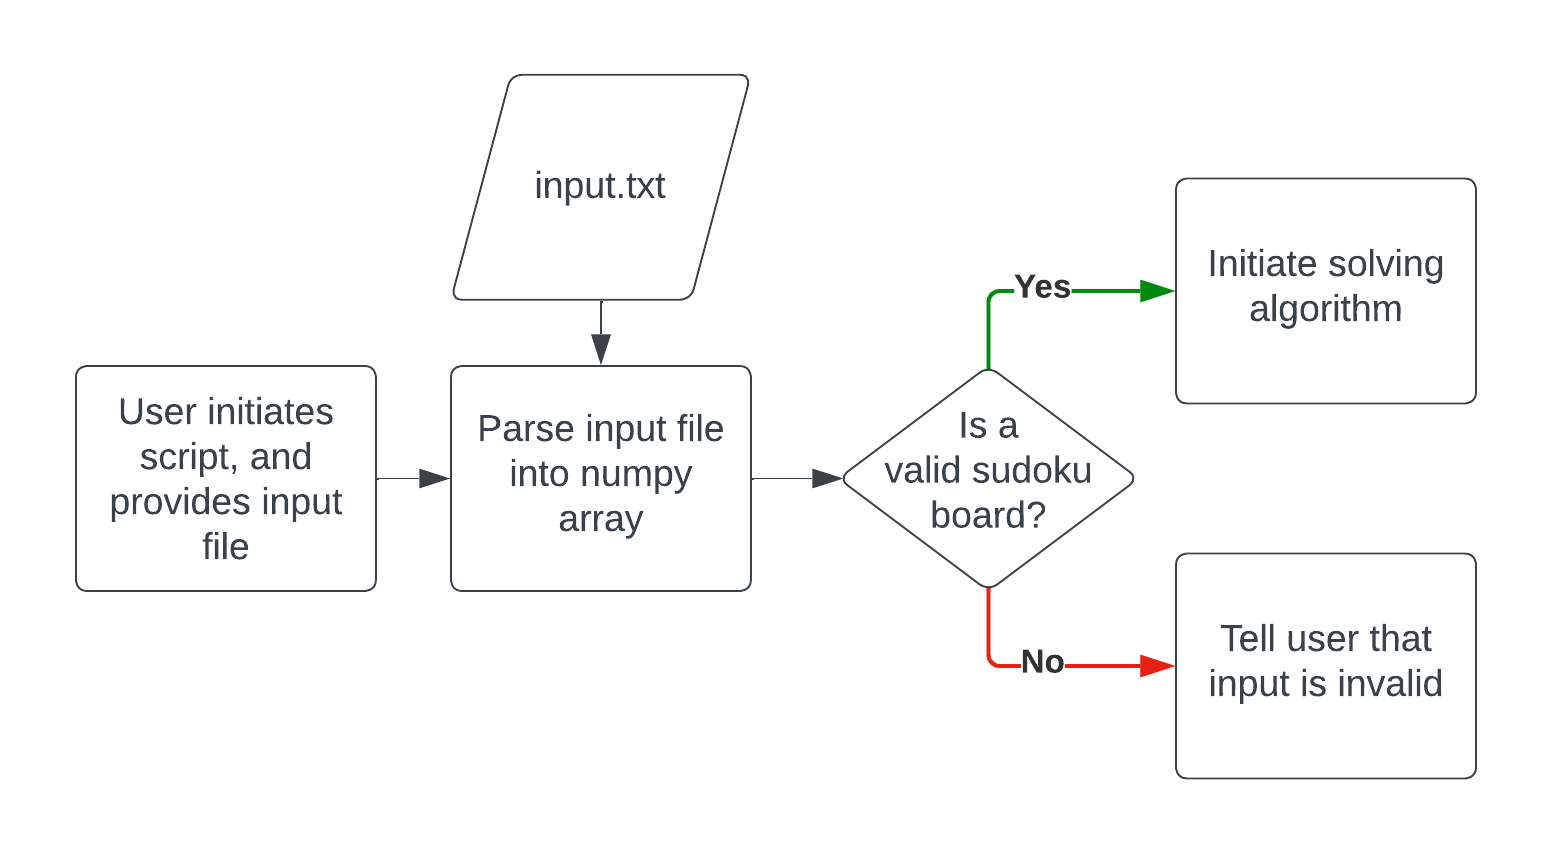
\includegraphics[width=0.9\textwidth]{./figures/parse-input-prototype}
    \caption{A flowchart for part 1 of solving a sudoku puzzle: parsing the user input.}
    \label{fig:input-prototype}
    \end{figure}

    \begin{figure}[htb]
    \centering
    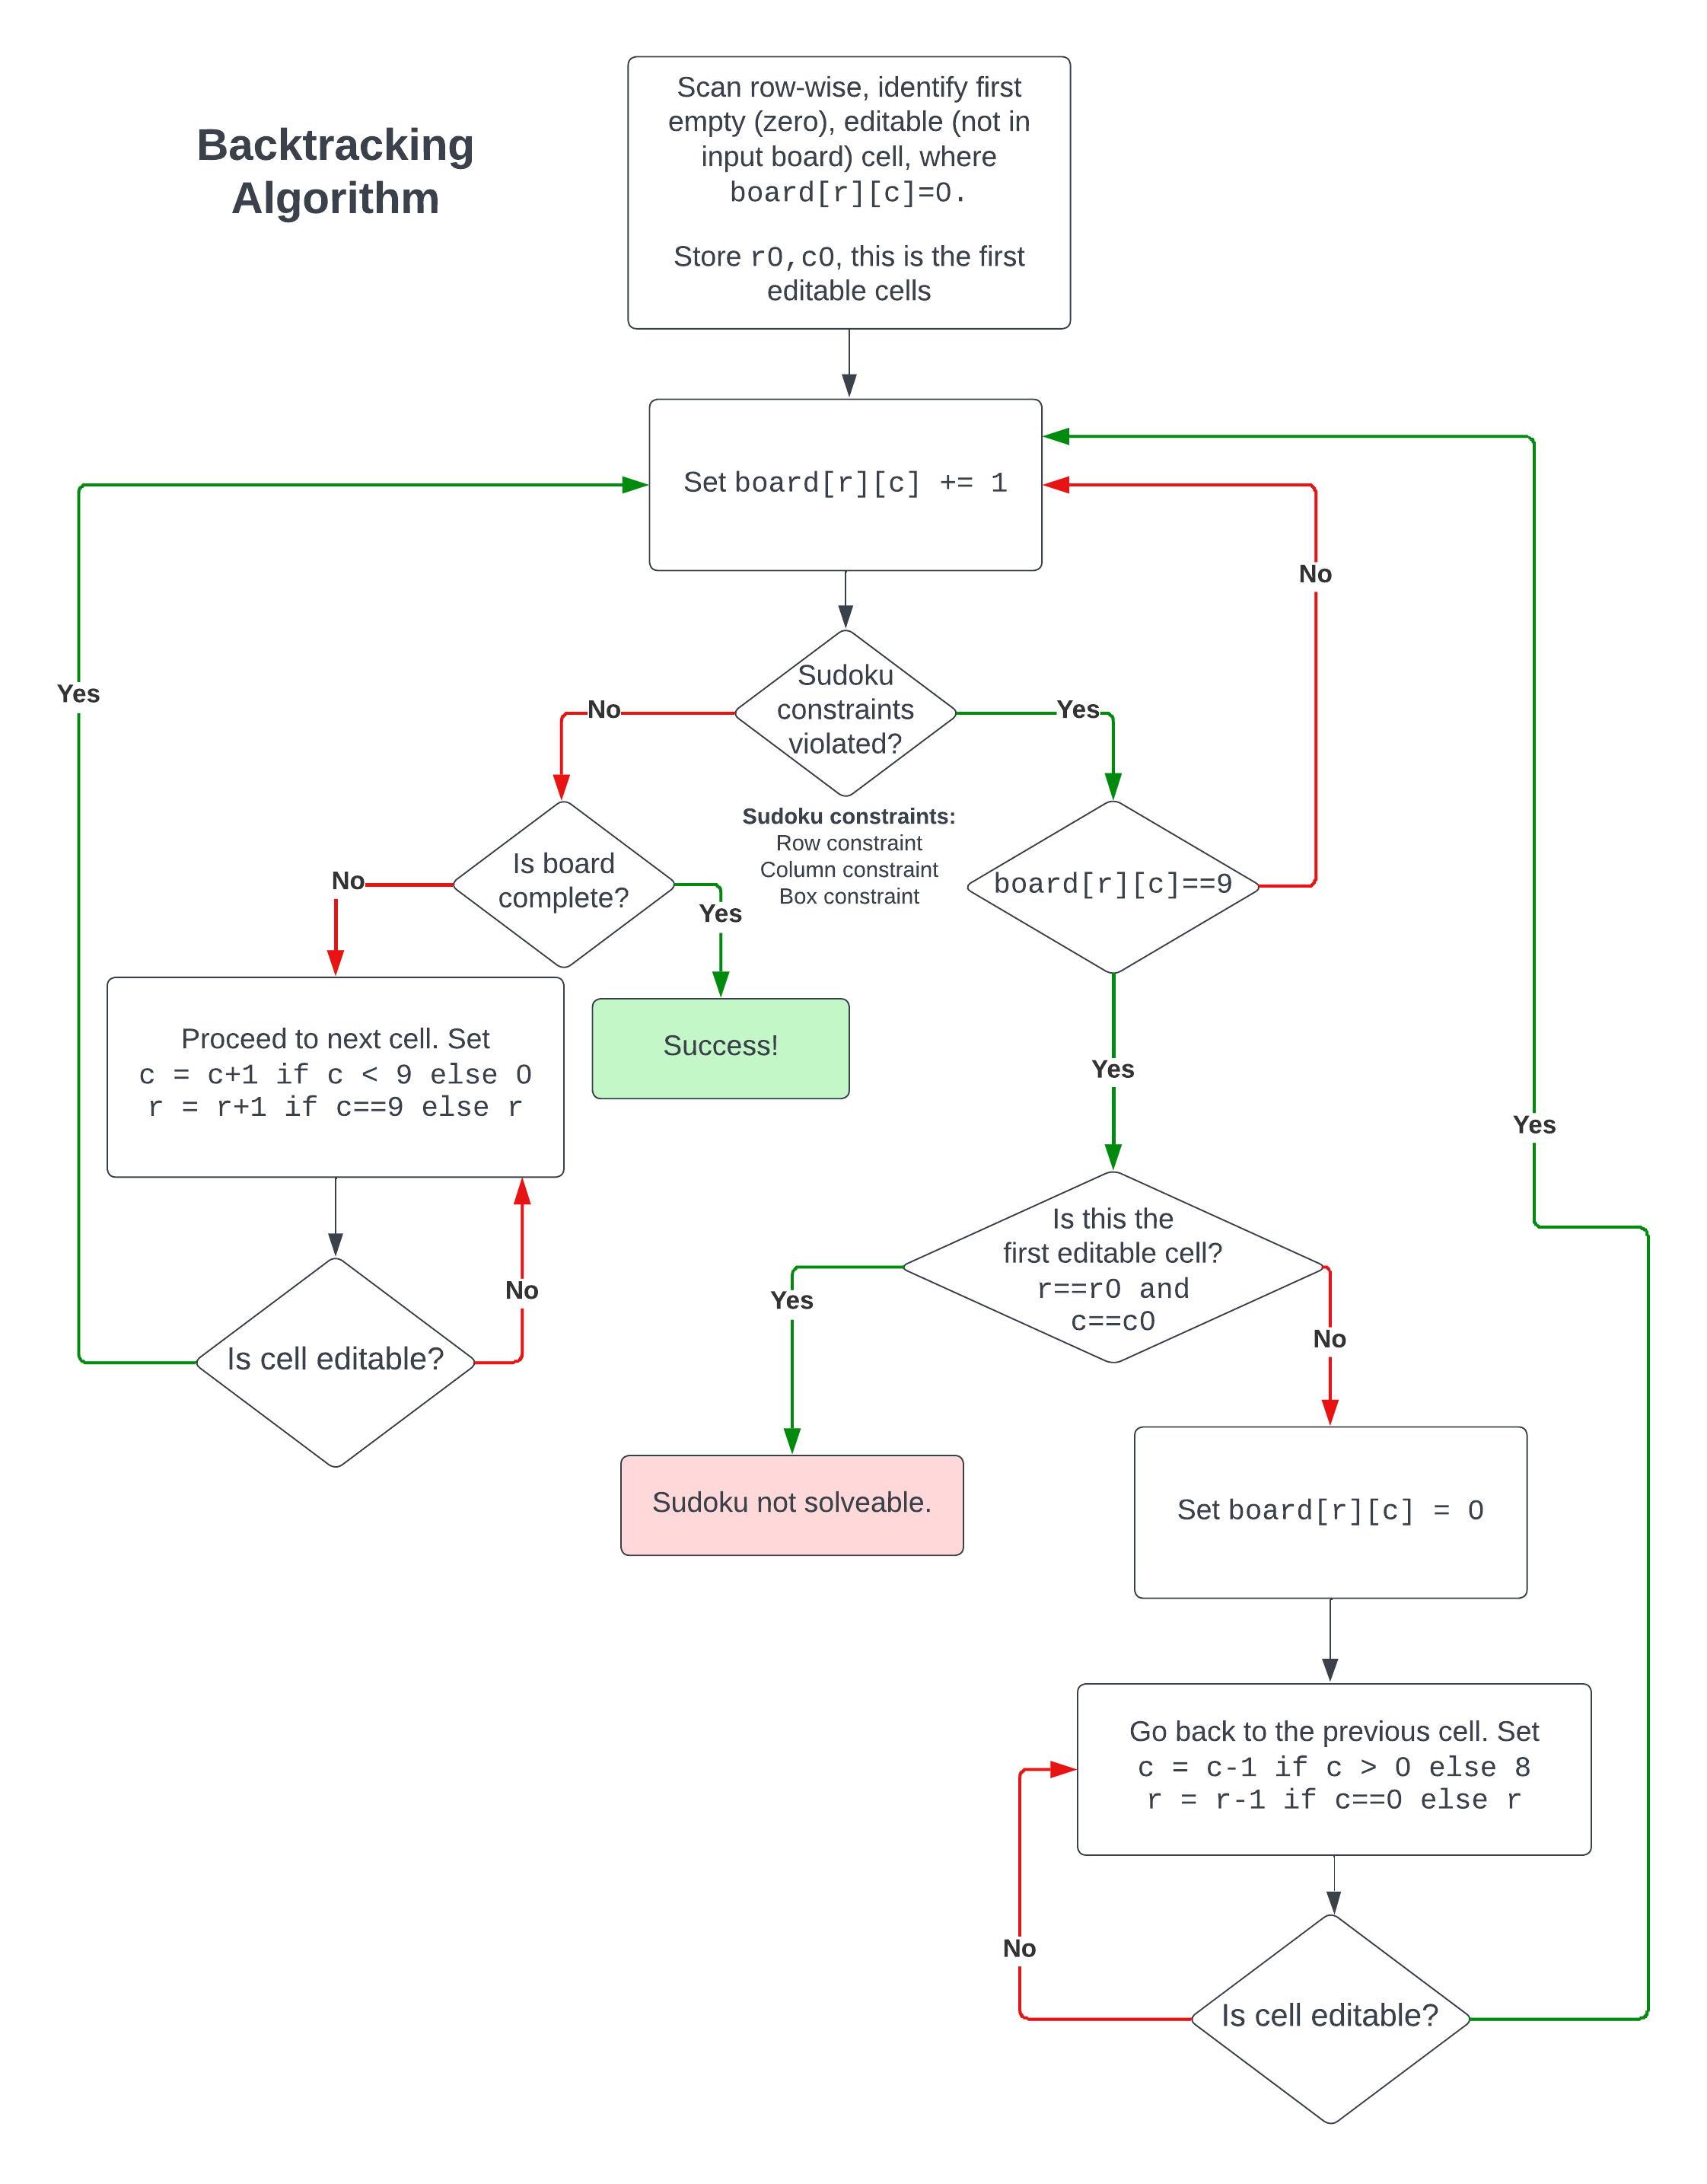
\includegraphics[width=0.9\textwidth]{./figures/backtracking-prototype}
    \caption{A flowchart for part 2 of solving a sudoku puzzle: the backtracking algorithm.}
    \label{fig:backtracking-prototype}
    \end{figure}

    \begin{figure}[htb]
    \centering
    \begin{lstlisting}[language=Python,label={lst:lstlisting}]
        class BacktrackingSolver
            def __init__(self, multiple_solutions: bool = False):
                self.board  # will store solved board
                self.is_solvable  # will store whether board is solvable
                self.is_solved  # will store whether board is solved
            def solve(self, unsolved_board: numpy.NDArray) -> None:

        def parse_input_file(input_file_path: str) -> numpy.NDArray

        def save_board(
            board: numpy.NDArray,
            output_file_path: str
        ) -> None

        # entry point for script, argv = sys.argv
        def handler(argv) -> None:
    \end{lstlisting}
    \caption{\textit{pseudo-python-code} representation of the interfaces of the functions and classes within our
    \inlinecode{sudokusolver} package.}
    \label{fig:pseudocode}
    \end{figure}
